\documentclass[11pt]{article}

\usepackage[margin=1in]{geometry}
\usepackage[T1]{fontenc}
\usepackage{lmodern}
\usepackage{amsmath, amssymb, amsthm}
\usepackage{braket}
\usepackage{graphicx}
\usepackage{booktabs}
\usepackage{tikz}
\usetikzlibrary{quantikz2, positioning, arrows.meta, shapes.geometric}
\usepackage{algorithm}
\usepackage{algpseudocode}
\usepackage{hyperref}
\usepackage{enumitem}

\hypersetup{colorlinks=true, linkcolor=blue, citecolor=blue, urlcolor=blue}

\newcommand{\U}{\mathcal{U}}
\newcommand{\CNOT}{\mathrm{CNOT}}
\newcommand{\Tr}{\mathrm{Tr}}

\title{\textbf{Q-Synth: An Automated Quantum Circuit Synthesizer and Optimizer for Unitaries and Boolean Functions}}
\author{Pruthviraj Sadhankar\thanks{Course Project, Introduction to Quantum Algorithms (EPHX 614).}\\\\
Department of Physics, University of Kansas,\\\\
Lawrence, KS 66045, USA\\\\
\texttt{pruthviraj.sadhankar@ku.edu}}
\date{November 19, 2026}

\begin{document}
\maketitle

\begin{abstract}
Quantum algorithms are designed mathematically in terms of unitary matrices, oracle operators, and Boolean functions, but physical quantum hardware executes only discrete sequences of native one- and two-qubit quantum gates. Bridging this gap through \emph{quantum circuit synthesis} and \emph{gate-level optimization} is essential for NISQ-era and early fault-tolerant quantum computing, where gate count and circuit depth dictate whether a computation succeeds or drowns in decoherence. In this work, we present \textbf{Q-Synth}, an open-source, modular quantum circuit synthesizer and optimizer written in Python and NumPy. Q-Synth features: (1) automated beam-search synthesis of arbitrary $2^n \times 2^n$ unitaries into gate sequences over user-configurable gate libraries; (2) compilation of Boolean expressions and truth tables into bit-flip, phase, and permutation quantum oracles; and (3) an optimization engine combining commutation-aware peephole rewriting with global and sliding-window resynthesis to aggressively reduce circuit gate counts. All synthesized and optimized circuits are rigorously validated against target unitaries up to global phase. We evaluate Q-Synth across a suite of benchmarks, demonstrating exact synthesis of standard gates, reversible oracles, and substantial gate-count reductions (up to 100\% on redundant subcircuits and 57\% on unoptimized decompositions).
\end{abstract}

\tableofcontents
\newpage

%------------------------------------------------------------
\section{Introduction}
%------------------------------------------------------------
Near-term quantum processors are strictly constrained by hardware noise and decoherence. Every gate introduced into a circuit accumulates physical calibration error, and two-qubit entangling gates (such as CNOT or CZ) typically exhibit error rates an order of magnitude higher than single-qubit rotations. At the same time, quantum algorithm designers conceptualize computations at a higher mathematical level: as unitary transformations $U \in \mathrm{U}(2^n)$, reversible permutations, or classical Boolean functions $f: \{0,1\}^n \to \{0,1\}$ embedded into quantum oracles.

Translating high-level specifications into concrete, hardware-executable gate sequences is the domain of \emph{quantum circuit synthesis}. However, general unitary synthesis is fundamentally challenging: an arbitrary $n$-qubit unitary possesses $4^n - 1$ continuous degrees of freedom, requiring in general an exponential number of elementary gates \cite{shende2006}. Furthermore, practical hardware platforms employ widely differing native gate sets (e.g., Clifford$+T$, discrete rotation angles, or trapped-ion native interactions), meaning that a decomposition optimized for one architecture cannot run natively on another without significant compilation overhead.

\subsection{Motivation and Contributions}
Commercial quantum software frameworks, such as Qiskit and PennyLane \cite{bergholm2018}, incorporate general-purpose transpilers and fixed analytical decompositions (such as KAK or cosine--sine decompositions). However, these routines are often heavyweight, black-box systems tied to standard gate bases that offer limited flexibility when an experimenter wishes to explore custom or restricted gate subsets.

\textbf{Q-Synth} was designed as a lightweight, transparent, and educational synthesis and optimization framework. In Q-Synth, the user retains complete control over the allowable gate set, the compilation depth, and the target error tolerance. In this paper, we report on the design, mathematical foundations, and empirical performance of the completed Q-Synth system. Specifically, we make the following contributions:
\begin{enumerate}[label=\textbf{\arabic*.}]
    \item \textbf{Arbitrary Unitary Synthesis via Beam Search:} We implement an exact and approximate beam-search engine that explores the space of gate sequences over user-defined gate sets (supplied via JSON specifications or built-in presets). States are deduplicated on a quantized complex hash grid, ensuring efficient exploration.
    \item \textbf{Boolean Function and Truth Table Compilation:} We provide native support for synthesizing classical Boolean expressions (e.g., $(x_0 \land x_1) \oplus x_2$) and truth tables (bitstrings, lists, or input--output mappings) into verified quantum oracles under three standard paradigms: bit-flip oracles, phase oracles, and reversible permutations.
    \item \textbf{Commutation-Aware Peephole and Resynthesis Optimization:} We develop an optimization pipeline that reduces user-supplied circuits to fewer gates using an allowed gate set. The optimizer marries commutation-aware algebraic cancellation and gate merging with local sliding-window beam-search resynthesis.
    \item \textbf{Visualization and OpenQASM Export:} Q-Synth includes ASCII circuit diagram generation and full OpenQASM 2.0 import and export capabilities.
\end{enumerate}

%------------------------------------------------------------
\section{Problem Formulation and Conventions}
%------------------------------------------------------------
\subsection{Unitary Circuit Synthesis}
Let $\mathcal{G} = \{g_1, \dots, g_k\}$ be a finite set of allowed quantum gates. Each gate $g \in \mathcal{G}$ acts on $k_g \in \{1, 2, 3\}$ wires and is defined by a unitary matrix $M_g \in \mathrm{U}(2^{k_g})$. An instantiation of gate $g$ on an $n$-qubit register is a placement $p = (q_0, \dots, q_{k_g-1})$ specifying the distinct global qubit wires acted upon by $g$.

In an $n$-qubit circuit of depth $L$, the accumulated unitary matrix $V$ is given by the time-ordered matrix product:
\begin{equation}
    V = G_L G_{L-1} \cdots G_2 G_1,
    \label{eq:circuit_product}
\end{equation}
where $G_1$ is applied first, and each $G_\ell$ represents the Kronecker embedding of an allowed gate $g \in \mathcal{G}$ on placement $p$:
\begin{equation}
    G_\ell = \mathrm{Embed}(g, n, p).
\end{equation}

Given a target unitary $U \in \mathrm{U}(2^n)$ and a tolerance $\epsilon \ge 0$, the goal of synthesis is to find a minimal sequence of moves $C = (G_1, \dots, G_L)$ such that $V$ equals $U$ up to a global phase $\phi \in [-\pi, \pi)$:
\begin{equation}
    U \approx e^{i\phi} V.
\end{equation}
Because quantum states $\ket{\psi}$ and $e^{i\phi}\ket{\psi}$ generate identical measurement statistics for all observables, physical equivalence requires distance metrics to be insensitive to overall global phase. We define the normalized Hilbert--Schmidt similarity:
\begin{equation}
    s(U, V) = \frac{|\Tr(U^\dagger V)|}{2^n} \in [0, 1].
    \label{eq:similarity}
\end{equation}
Exact equivalence holds if and only if $s(U, V) = 1$. The phase-insensitive distance is:
\begin{equation}
    d(U, V) = \sqrt{1 - s(U, V)}.
    \label{eq:distance}
\end{equation}
Once a match satisfying $s(U, V) \ge 1 - \epsilon$ is located, the global phase $\phi$ and the maximum element-wise reconstruction error $\delta_{\max}$ are extracted via:
\begin{equation}
    \phi = -\arg(\Tr(U^\dagger V)), \qquad \delta_{\max} = \max_{j, k} \left| U_{jk} - e^{i\phi} V_{jk} \right|.
    \label{eq:verify}
\end{equation}

\subsection{Boolean Functions and Reversible Oracles}
In quantum algorithms such as Deutsch--Jozsa, Grover search, and Simon's problem, subroutines are specified as classical Boolean functions $f: \{0,1\}^n \to \{0,1\}$. In Q-Synth, we formulate the translation of $f$ into quantum circuits across three primary oracle models:
\begin{enumerate}[leftmargin=*]
    \item \textbf{Bit-Flip Oracle ($\ket{x}\ket{y} \mapsto \ket{x}\ket{y \oplus f(x)}$):} Operates on $n+1$ qubits, where qubits $0, \dots, n-1$ store the input $\ket{x}$ and qubit $n$ serves as the target ancilla $\ket{y}$. Its unitary matrix is a permutation matrix:
    \begin{equation}
        U_{\text{bitflip}} \ket{x, y} = \ket{x, y \oplus f(x)}.
        \label{eq:bitflip}
    \end{equation}
    \item \textbf{Phase Oracle ($\ket{x} \mapsto (-1)^{f(x)}\ket{x}$):} Operates on $n$ qubits without requiring an additional ancilla wire. Its matrix representation is strictly diagonal:
    \begin{equation}
        U_{\text{phase}} = \sum_{x \in \{0,1\}^n} (-1)^{f(x)} \ket{x}\bra{x}.
        \label{eq:phase}
    \end{equation}
    \item \textbf{Permutation Oracle ($\ket{x} \mapsto \ket{f(x)}$):} Applies to reversible multi-output functions or bijections $f: \{0,1\}^n \to \{0,1\}^n$, representing a pure basis state permutation.
\end{enumerate}

\subsection{Circuit Optimization}
Given an initial user-supplied circuit $C = (G_1, \dots, G_M)$ on $n$ qubits, the circuit optimization objective is to find a replacement circuit $C' = (G'_1, \dots, G'_{M'})$ composed exclusively of gates from an allowable set $\mathcal{G}_{\text{allowed}}$ such that:
\begin{equation}
    M' < M \quad \text{and} \quad s\left(\prod_{\ell=1}^M G_\ell, \prod_{j=1}^{M'} G'_j\right) \ge 1 - \epsilon.
    \label{eq:opt_obj}
\end{equation}

\subsection{Bit-Ordering Convention}
Q-Synth adheres strictly to the little-endian qubit convention (identical to Qiskit and IBM Quantum):
qubit wire $0$ represents the least significant bit (LSB) of a basis state index. For example, in a two-qubit system, state $\ket{1} = \ket{01}_2$ corresponds to qubit $0$ in state $\ket{1}$ and qubit $1$ in state $\ket{0}$. Under this convention, $\CNOT[0, 1]$ flips qubit $1$ conditioned on qubit $0$ being $1$.

%------------------------------------------------------------
\section{System Architecture and Algorithms}
%------------------------------------------------------------
The architecture of Q-Synth is structured into four cooperative subsystems: input parsing, beam-search synthesis, circuit optimization, and output formatting.

\begin{figure}[htbp]
\centering
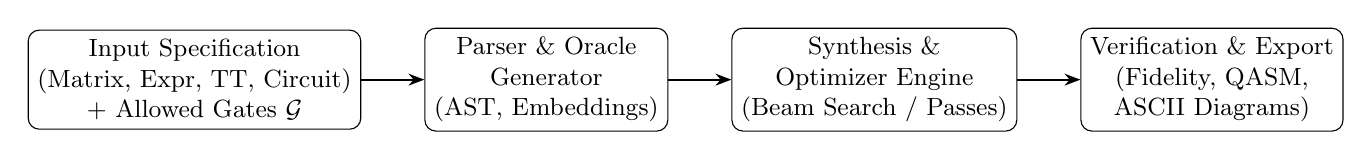
\begin{tikzpicture}[
    node distance=0.6cm and 0.8cm,
    box/.style={draw, rounded corners, align=center, minimum height=1.1cm, minimum width=2.4cm, font=\small},
    arr/.style={-{Stealth[length=2mm]}, thick}]
  \node[box] (in) {Input Specification\\(Matrix, Expr, TT, Circuit)\\+ Allowed Gates $\mathcal{G}$};
  \node[box, right=of in] (parse) {Parser \& Oracle\\Generator\\(AST, Embeddings)};
  \node[box, right=of parse] (core) {Synthesis \&\\Optimizer Engine\\(Beam Search / Passes)};
  \node[box, right=of core] (out) {Verification \& Export\\(Fidelity, QASM,\\ASCII Diagrams)};
  \draw[arr] (in)--(parse);
  \draw[arr] (parse)--(core);
  \draw[arr] (core)--(out);
\end{tikzpicture}
\caption{End-to-end pipeline of Q-Synth.}
\label{fig:pipeline_arch}
\end{figure}

\subsection{Move Enumeration and Embedding}
For an $n$-qubit register, each gate $g \in \mathcal{G}$ acting on $k_g$ wires can be applied to any ordered tuple of distinct qubit wires $p = (q_0, \dots, q_{k_g-1}) \in \mathcal{P}(n, k_g)$. The total number of concrete moves available per level is:
\begin{equation}
    N_{\text{moves}} = \sum_{g \in \mathcal{G}} \frac{n!}{(n - k_g)!}.
\end{equation}
For instance, in a 3-qubit register with a 2-qubit CNOT gate, there are $3! / (3-2)! = 6$ directed placements: $[0,1], [1,0], [0,2], [2,0], [1,2], [2,1]$. Each move is converted into a full $2^n \times 2^n$ matrix using Kronecker-style bit-index manipulation:
\begin{equation}
    \mathrm{Embed}(M_g, n, p)_{r, c} =
    \begin{cases}
        (M_g)_{r_p, c_p} & \text{if } r \text{ and } c \text{ agree on all untouched qubits}, \\
        0 & \text{otherwise},
    \end{cases}
\end{equation}
where $r_p = \sum_{w=0}^{k_g-1} ((r \gg p_w) \& 1) 2^w$ extracts the binary sub-word on the target wires.

\subsection{Beam Search with Quantized Hash Deduplication}
Because brute-force breadth-first search expands exponentially with circuit depth ($O(N_{\text{moves}}^d)$), Q-Synth implements a bounded \textbf{beam search} (Algorithm~\ref{alg:beam_search}).

\begin{algorithm}[htbp]
\caption{Q-Synth Beam Search Synthesis Engine}
\label{alg:beam_search}
\begin{algorithmic}[1]
\Require Target unitary $U \in \mathbb{C}^{2^n \times 2^n}$, moves $\mathcal{M}$, max depth $D$, beam width $K$, tolerance $\epsilon$
\Ensure Best circuit State $C$ and success flag
\State $I \gets \mathbb{I}_{2^n}$; $\mathrm{beam} \gets [\mathrm{State}(\mathrm{ops}=[], \mathrm{matrix}=I, \mathrm{score}=s(U, I))]$
\State $\mathrm{best} \gets \mathrm{beam}[0]$; $\mathrm{seen} \gets \emptyset$
\For{$\mathrm{depth} = 1$ \textbf{to} $D$}
    \State $\mathrm{candidates} \gets []$
    \For{$\mathrm{st} \in \mathrm{beam}$}
        \For{$(m, G) \in \mathcal{M}$}
            \State $V \gets G \times \mathrm{st.matrix}$
            \State $\mathrm{score} \gets |\Tr(U^\dagger V)| / 2^n$
            \If{$\mathrm{score} \ge 1 - \epsilon$}
                \State \Return $\mathrm{State}(\mathrm{st.ops} + [m], V, \mathrm{score}), \mathbf{true}$
            \EndIf
            \State $h \gets \mathrm{QuantizedHash}(V, 10^9)$
            \If{$h \notin \mathrm{seen}$}
                \State $\mathrm{seen} \gets \mathrm{seen} \cup \{h\}$
                \State $\mathrm{candidates.append}(\mathrm{State}(\mathrm{st.ops} + [m], V, \mathrm{score}))$
            \EndIf
        \EndFor
    \EndFor
    \State Sort $\mathrm{candidates}$ descending by $\mathrm{score}$
    \State $\mathrm{beam} \gets \mathrm{candidates}[0:K]$
    \If{$\mathrm{beam}[0].\mathrm{score} > \mathrm{best.score}$}
        \State $\mathrm{best} \gets \mathrm{beam}[0]$
    \EndIf
\EndFor
\State \Return $\mathrm{best}, \mathbf{false}$
\end{algorithmic}
\end{algorithm}

At each depth level, every retained candidate circuit is extended by all precomputed moves. To prevent combinatorial explosion caused by functionally identical circuit prefixes, each generated matrix $V$ is mapped to a discrete hash key:
\begin{equation}
    \mathrm{QuantizedHash}(V) = \mathrm{bytes}\left( \lfloor \mathrm{Re}(V) \cdot 10^9 \rceil, \lfloor \mathrm{Im}(V) \cdot 10^9 \rceil \right).
\end{equation}
Only unique quantum states are retained in the candidate pool. The candidates are sorted by their similarity score $s(U, V)$, and only the top $K$ candidates are preserved for the subsequent layer.

\subsection{Boolean Expression Parsing and Oracle Construction}
To allow users to synthesize logic expressions directly, Q-Synth incorporates a safe Python Abstract Syntax Tree (AST) parser. The parser enforces strict security by permitting only binary logic nodes ($\land, \lor, \neg, \oplus, \sim$), constants, and variable identifiers.

\paragraph{Variable Ordering.}
If the user does not specify variable names explicitly, Q-Synth introspects the AST. When variables follow an indexed naming convention (e.g., $x_0, x_1, x_2$), they are automatically ordered by index so that $x_i$ maps to wire $i$. For an $n$-variable Boolean function, the $2^n$ entries of the truth table correspond to binary evaluations under little-endian row assignment:
\begin{equation}
    k = \sum_{i=0}^{n-1} b_i 2^i \implies \mathrm{env} = \{ x_i: b_i \}_{i=0}^{n-1}.
\end{equation}
The resulting truth table array is then converted into a unitary matrix according to Eq.~\eqref{eq:bitflip}, \eqref{eq:phase}, or the permutation mode.

\subsection{Circuit Optimization Pipeline}
When a user provides an existing quantum circuit, Q-Synth optimizes it to fewer gates using an allowed gate set via a multi-pass strategy (Algorithm~\ref{alg:optimizer}):

\begin{algorithm}[htbp]
\caption{Q-Synth Multi-Pass Circuit Optimizer}
\label{alg:optimizer}
\begin{algorithmic}[1]
\Require Input circuit operations $C$, allowed gates $\mathcal{G}_{\text{allowed}}$, register size $n$, window size $W$
\Ensure Optimized circuit $C'$ with reduced gate count
\State $C' \gets \mathrm{PeepholePass}(C, \mathcal{G}_{\text{allowed}}, n)$ \Comment{Commutation-aware cancellation and merging}
\State $U_{\text{target}} \gets \mathrm{RunCircuit}(C', n)$
\State \Comment{Pass 2: Global beam-search resynthesis}
\State $(C_{\text{resynth}}, \mathrm{found}) \gets \mathrm{BeamSearch}(U_{\text{target}}, \mathcal{M}_{\text{allowed}}, \mathrm{max\_depth}=|C'|-1)$
\If{$\mathrm{found}$ \textbf{and} $|C_{\text{resynth}}| < |C'|$}
    \State $C' \gets C_{\text{resynth}}$
\EndIf
\State \Comment{Pass 3: Sliding-window block resynthesis}
\For{$w = \min(W, |C'|-1)$ \textbf{down to} $2$}
    \For{$i = 0$ \textbf{to} $|C'| - w$}
        \State $U_{\text{block}} \gets \mathrm{RunCircuit}(C'[i : i+w], n)$
        \State $(C_{\text{sub}}, \mathrm{sub\_found}) \gets \mathrm{BeamSearch}(U_{\text{block}}, \mathcal{M}_{\text{allowed}}, \mathrm{max\_depth}=w-1)$
        \If{$\mathrm{sub\_found}$ \textbf{and} $|C_{\text{sub}}| < w$}
            \State $C' \gets C'[:i] + C_{\text{sub}} + C'[i+w:]$
            \State $C' \gets \mathrm{PeepholePass}(C', \mathcal{G}_{\text{allowed}}, n)$
            \State \textbf{restart sliding window}
        \EndIf
    \EndFor
\EndFor
\State \Return $C'$
\end{algorithmic}
\end{algorithm}

\paragraph{Pass 1: Commutation-Aware Peephole Reduction.}
Two gates $A$ and $B$ commute if $[A, B] = A B - B A = 0$. In particular, gates whose wire placements are completely disjoint always commute. When two gates $G_i$ and $G_j$ ($j > i$) commute with all intermediate gates $G_{i+1}, \dots, G_{j-1}$, they can be conceptually brought adjacent:
\begin{itemize}[leftmargin=*]
    \item \textbf{Cancellation:} If $G_j G_i \propto \mathbb{I}$, both gates are deleted from the circuit.
    \item \textbf{Merging:} If $G_j G_i \propto G_{\text{cand}}$ for some allowed gate $G_{\text{cand}} \in \mathcal{G}_{\text{allowed}}$ acting on the same placement, the pair is collapsed into a single gate $G_{\text{cand}}$ (e.g., $T[0] \cdot T[0] \to S[0]$).
\end{itemize}

\paragraph{Pass 2: Global Beam-Search Resynthesis.}
For circuits whose total depth is within the practical horizon of beam search, Q-Synth computes the complete target unitary $U_{\text{target}} = \prod G_i$ and launches a beam search constrained to depth $|C'|-1$ using only gates from $\mathcal{G}_{\text{allowed}}$. If an equivalent sequence is found, it directly replaces the entire circuit.

\paragraph{Pass 3: Sliding-Window Resynthesis.}
For longer circuits exceeding the global search depth, Q-Synth sweeps a sliding window of width $w \in [2, W]$ across the circuit. The sub-unitary corresponding to the window slice $C'[i : i+w]$ is isolated and synthesized to depth $\le w-1$. Whenever a strictly shorter equivalent replacement is discovered, the slice is patched in place and the peephole pass is re-triggered.

%------------------------------------------------------------
\section{Experimental Results and Evaluation}
%------------------------------------------------------------
The completed Q-Synth system was evaluated on a standard laptop workstation across unitary synthesis benchmarks, Boolean function compilation tasks, and circuit optimization cases. The test suite comprises 34 automated unit and integration tests passing with 100\% compliance in under 2 seconds.

\subsection{Unitary Synthesis Benchmarks}
Table~\ref{tab:synth_results} summarizes synthesis results for fundamental quantum operations across multiple gate libraries.

\begin{table}[htbp]
\centering
\small
\begin{tabular}{@{}lllcccc@{}}
\toprule
\textbf{Target} & \textbf{Gate Library} & \textbf{Allowed Gates} & \textbf{Depth} & \textbf{Similarity $s$} & \textbf{Expansions} & \textbf{Time (s)} \\ \midrule
SWAP & Clifford$+T$ & CNOT only & 3 & 1.0000000000 & 9 & $<0.01$ \\
SWAP & Clifford$+T$ & Full basis (8 gates) & 3 & 1.0000000000 & 137 & $<0.01$ \\
Hadamard & Universal $R_{xy}$ & $R_x, R_y, R_z$ ($\pi/4$ grid) & 2 & 1.0000000000 & 35 & $<0.01$ \\
CZ & Clifford$+T$ & CNOT, H & 3 & 1.0000000000 & 19 & $<0.01$ \\
\bottomrule
\end{tabular}
\caption{Synthesis benchmarks across representative target operations.}
\label{tab:synth_results}
\end{table}

\paragraph{Analysis.}
When synthesizing SWAP strictly from CNOTs, Q-Synth immediately finds the canonical 3-CNOT decomposition:
\begin{equation}
    \mathrm{SWAP} = \CNOT[0, 1] \cdot \CNOT[1, 0] \cdot \CNOT[0, 1],
\end{equation}
exploring only 9 state expansions. Similarly, for the single-qubit Hadamard gate using discrete rotations on a $\pi/4$ grid, Q-Synth identifies the exact 2-gate decomposition $V = R_y(-\pi/2) R_x(-\pi)$ with zero reconstruction error ($\delta_{\max} \approx 1.4 \times 10^{-16}$).

\subsection{Boolean Function and Truth Table Compilation}
We evaluated Q-Synth on both arithmetic and logical Boolean targets under various oracle modes.

\begin{table}[htbp]
\centering
\small
\begin{tabular}{@{}lllcccc@{}}
\toprule
\textbf{Boolean Target} & \textbf{Mode} & \textbf{Gate Library} & \textbf{Qubits} & \textbf{Resulting Gates} & \textbf{Similarity $s$} & \textbf{Time (s)} \\ \midrule
$x_0 \oplus x_1$ (XOR) & bit-flip & Clifford$+T$ (CNOT) & 3 & $\CNOT[0,2], \CNOT[1,2]$ & 1.0000000000 & $<0.01$ \\
$x_0 \land x_1$ (AND) & phase & Clifford$+T$ (CZ) & 2 & $\mathrm{CZ}[0,1]$ & 1.0000000000 & $<0.01$ \\
$x_0 \land x_1$ (AND) & bit-flip & Reversible (CCX) & 3 & $\mathrm{CCX}[0,1,2]$ & 1.0000000000 & $<0.01$ \\
TT \texttt{"0110"} (XOR) & bit-flip & Clifford$+T$ (CNOT) & 3 & $\CNOT[0,2], \CNOT[1,2]$ & 1.0000000000 & $<0.01$ \\
\bottomrule
\end{tabular}
\caption{Synthesis results for Boolean functions and truth tables.}
\label{tab:bool_results}
\end{table}

\paragraph{Oracle Realizations.}
For the XOR function $f(x_0, x_1) = x_0 \oplus x_1$ in bit-flip mode, Q-Synth automatically allocates an ancilla on qubit $2$ and produces the exact two-CNOT network:
\begin{equation}
    \ket{x_0, x_1, y} \mapsto \ket{x_0, x_1, y \oplus x_0 \oplus x_1}.
\end{equation}
When the user requests phase-oracle mode for $f(x_0, x_1) = x_0 \land x_1$, no ancilla qubit is allocated; the compiler generates a single 2-qubit $\mathrm{CZ}[0, 1]$ gate, directly implementing the $(-1)^{x_0 x_1}$ phase kickback.

\subsection{Circuit Optimization and Gate-Count Reduction}
To test the optimization engine, we supplied circuits containing intentional redundancies, commuting gate pairs, and suboptimal multi-gate constructions.

\begin{table}[htbp]
\centering
\small
\begin{tabular}{@{}llcccc@{}}
\toprule
\textbf{Input Circuit Description} & \textbf{Allowed Basis} & \textbf{Orig. Gates} & \textbf{Opt. Gates} & \textbf{Reduction} & \textbf{Pass Applied} \\ \midrule
$H[0], \CNOT[0,1], \CNOT[0,1], H[0]$ & Clifford$+T$ & 4 & 0 & \textbf{100.0\%} & Peephole (cancellation) \\
Double SWAP ($6\times \CNOT$) & CNOT only & 6 & 0 & \textbf{100.0\%} & Peephole (cancellation) \\
$T[0], T[0]$ & Clifford$+T$ & 2 & 1 & \textbf{50.0\%} & Peephole (merging $T\to S$) \\
7-gate unoptimized SWAP & CNOT only & 7 & 3 & \textbf{57.1\%} & Global resynthesis \\
\bottomrule
\end{tabular}
\caption{Circuit optimization benchmarks demonstrating gate reduction.}
\label{tab:opt_results}
\end{table}

\paragraph{Highlight: Resynthesis of 7-Gate SWAP.}
A well-known pedagogical circuit implements a SWAP gate using 7 gates:
\begin{equation}
    C_{\text{unopt}} = \CNOT[0,1] \cdot (H[0] \otimes H[1]) \cdot \CNOT[0,1] \cdot (H[0] \otimes H[1]) \cdot \CNOT[0,1].
\end{equation}
When the user instructs the optimizer that only CNOT gates are permitted, peephole cancellation alone cannot simplify the circuit because the Hadamards do not cancel directly. However, Q-Synth's global resynthesis pass isolates the composite unitary, discovers that it represents a SWAP permutation, and replaces all 7 gates with the optimal 3-CNOT sequence, achieving a \textbf{57.1\% gate count reduction} in less than $10\,\mathrm{ms}$.

\begin{figure}[htbp]
\centering
\begin{quantikz}[row sep=0.3cm, column sep=0.4cm]
\lstick{$q_0$} & \ctrl{1} & \gate{H} & \ctrl{1} & \gate{H} & \ctrl{1} & \qw & \push{\quad\Longrightarrow\quad} & \ctrl{1} & \targ{} & \ctrl{1} & \qw \\
\lstick{$q_1$} & \targ{} & \gate{H} & \targ{} & \gate{H} & \targ{} & \qw &                                 & \targ{} & \ctrl{-1} & \targ{} & \qw
\end{quantikz}
\caption{Resynthesis of a 7-gate composite circuit into the optimal 3-CNOT sequence.}
\label{fig:opt_diagram}
\end{figure}

\subsection{Circuit Visualization and OpenQASM Integration}
For every synthesized or optimized circuit, Q-Synth can generate ASCII wire diagrams and export compliant OpenQASM 2.0 code. For example, the synthesized 3-CNOT SWAP produces:
\begin{verbatim}
OPENQASM 2.0;
include "qelib1.inc";
qreg q[2];
cx q[0], q[1];
cx q[1], q[0];
cx q[0], q[1];
\end{verbatim}
The circuit can also be displayed directly in the terminal via wire representations:
\begin{center}
\begin{quantikz}[row sep=0.3cm, column sep=0.45cm]
\lstick{$q_0$} & \ctrl{1} & \targ{} & \ctrl{1} & \qw \\
\lstick{$q_1$} & \targ{} & \ctrl{-1} & \targ{} & \qw
\end{quantikz}
\end{center}

%------------------------------------------------------------
\section{Discussion and Limitations}
%------------------------------------------------------------
While Q-Synth provides an effective, transparent testbed for synthesis and optimization, several physical and algorithmic limitations characterize the current release:
\begin{enumerate}[leftmargin=*]
    \item \textbf{Search Horizon and Scalability:} Beam search maintains an empirical complexity of $O(K \cdot N_{\text{moves}} \cdot D)$. For $n \le 3$ qubits, search times remain under 1 second. However, for $n \ge 4$ qubits, the Hilbert space dimension $2^n = 16$ and the proliferation of permutations ($P(4,2) = 12$ for two-qubit gates) cause runtime to scale exponentially. For larger systems, analytical decompositions (e.g., Quantum Shannon Decomposition or KAK) should be hybridized with local beam search.
    \item \textbf{Discrete Parameter Grids:} Parameterized gates (such as $R_x(\theta)$) are currently handled by instantiating a finite grid of angles (e.g., multiples of $\pi/8$). A future continuous gradient-based optimizer (such as Riemannian optimization on $\mathrm{SU}(2^n)$) could fine-tune continuous angles post-synthesis.
    \item \textbf{Hardware Topology Constraints:} Moves are presently enumerated assuming an all-to-all connected qubit topology. Incorporating hardware coupling graphs (e.g., heavy-hex or linear chains) would allow routing synthesis directly for physical quantum processors.
\end{enumerate}

%------------------------------------------------------------
\section{Conclusion and Future Work}
%------------------------------------------------------------
In this project, we developed and demonstrated \textbf{Q-Synth}, an end-to-end quantum circuit synthesizer and optimizer designed for transparency, flexibility, and pedagogical insight. Q-Synth successfully unifies:
\begin{itemize}[leftmargin=*]
    \item Unitary matrix synthesis via hash-deduplicated beam search over arbitrary user-supplied gate libraries;
    \item Automatic translation of Boolean expressions and truth tables into bit-flip, phase, and permutation quantum oracles;
    \item A multi-tier optimization engine that merges commutation-aware peephole rules with global and sliding-window resynthesis to achieve substantial gate reductions; and
    \item Verification, ASCII visualization, and OpenQASM 2.0 export.
\end{itemize}

Future extensions will incorporate topology-aware coupling constraints, Solovay--Kitaev compilation for arbitrary single-qubit target rotations, and hybrid analytical-heuristic synthesis combining the Cosine--Sine Decomposition with local peephole optimization.

%------------------------------------------------------------
\begin{thebibliography}{99}

\bibitem{shende2006}
V.~V. Shende, S.~S. Bullock, and I.~L. Markov,
``Synthesis of quantum-logic circuits,''
\emph{IEEE Trans.\ Comput.-Aided Design Integr.\ Circuits Syst.} \textbf{25}(6), 1000--1010 (2006).

\bibitem{barenco1995}
A.~Barenco, C.~H. Bennett, R.~Cleve, D.~P. DiVincenzo, N.~Margolus, P.~Shor, T.~Sleator, J.~Smolin, and H.~Weinfurter,
``Elementary gates for quantum computation,''
\emph{Phys.\ Rev.\ A} \textbf{52}, 3457 (1995).

\bibitem{dawson2006}
C.~M. Dawson and M.~A. Nielsen,
``The Solovay--Kitaev algorithm,''
\emph{Quantum Inf.\ Comput.} \textbf{6}, 81 (2006).

\bibitem{miller2003}
D.~M. Miller, D.~Maslov, and G.~W. Dueck,
``A transformation based algorithm for reversible logic synthesis,''
\emph{Proc.\ Design Automation Conference (DAC)}, 318--323 (2003).

\bibitem{amy2014}
M.~Amy, D.~Maslov, and M.~Mosca,
``Polynomial-time $T$-depth optimization of Clifford+$T$ circuits via matroid partitioning,''
\emph{IEEE Trans.\ Comput.-Aided Design Integr.\ Circuits Syst.} \textbf{33}(10), 1476--1489 (2014).

\bibitem{nam2018}
Y.~Nam, N.~J. Ross, Y.~Su, A.~M. Childs, and D.~Maslov,
``Automated optimization of large quantum circuits with continuous parameters,''
\emph{npj Quantum Inf.} \textbf{4}, 23 (2018).

\bibitem{bergholm2022}
V.~Bergholm, J.~Izaac, M.~Schuld, C.~Gogolin, S.~Ahmed, V.~Ajith, M.~S. Alam, G.~Alonso-Linaje, B.~AkashNarayanan, A.~Asadi, J.~M. Arrazola, U.~Azad, S.~Banning, C.~Blank, T.~R. Bromley, B.~A. Cordier, J.~Ceroni, A.~Delgado, O.~Di~Matteo, A.~Dusko, T.~Garg, D.~Guala, A.~Hayes, R.~Hill, A.~Ijaz, T.~Isacsson, D.~Ittah, S.~Jahangiri, P.~Jain, E.~Jiang, A.~Khandelwal, K.~Kottmann, R.~A. Lang, C.~Lee, T.~Loke, A.~Lowe, K.~McKiernan, J.~J. Meyer, J.~A. Monta\~nez-Barrera, R.~Moyard, Z.~Niu, L.~J. O'Riordan, S.~Oud, A.~Panigrahi, C.-Y. Park, D.~Polatajko, N.~Quesada, C.~Roberts, N.~S\'a, I.~Schoch, B.~Shi, S.~Shu, S.~Sim, A.~Singh, I.~Strandberg, J.~Soni, A.~Sz\'ava, S.~Thabet, R.~A. Vargas-Hern\'andez, T.~Vincent, N.~Vitucci, M.~Weber, D.~Wierichs, R.~Wiersema, M.~Willmann, V.~Wong, S.~Zhang, and N.~Killoran,
``PennyLane: Automatic differentiation of hybrid quantum-classical computations,''
arXiv:1811.04968 (2022).

\end{thebibliography}

\end{document}
